%!TEX root = thesis.tex

\chapter{Preliminaries}

	In this chapter we present up the formal definitions we will need for the rest of the thesis. These serve as a reference and an introduction to the technical work we have done in the following chapters. These definitions naturally lead into a few foundational lemmas which will be presented at the end of the chapter. Some definitions are very basic indeed and many will already be known to the reader, and so they are stated explicitly here simply to provide maximum clarity and a solid foundation upon which to present the rest of our work.

	For additional definitions which are out of the scope of this thesis the reader may refer to textbooks on set theory \cite{kunen1980set} and lattice theory \cite{birkhoff1995lattice}.

\section{Definitions}

	\begin{definition}
		A \emph{permutation} of a set $X$ is a bijective function from $X$ to $X$.
	\end{definition}

	\begin{definition}
		A \emph{total ordering} over a set $X$ is a binary relation on $X$ which is antisymmetric, transitive, and total.
	\end{definition}

	Although technically permutations and total orderings are different constructs (bijective functions versus binary relations), they often have similar applications. For example, given a totally-ordered set $X$ and a permutation $\sigma$ on $X$, we can construct a total ordering $R = \{(x,y) \mid x, y \in X, \sigma^{-1}(x) < \sigma^{-1}(y)\}$ which is similar to $\sigma$. Likewise, one could construct $\sigma$ from $R$ where $\sigma : X \to X$ such that $\sigma(x) = y$ iff $\forall z \in X, z < x \implies z < y$.

	For countable sets we will sometimes view permutations and total orders as sequences of elements, using a subscript notation, provided our meaning is clear from context.

	\begin{definition}
		We use $S(X)$ to denote the set of all permutations of $X$.
	\end{definition}

	\begin{definition}
		We use $L(X)$ to denote the set of all total orders over $X$.
	\end{definition}

	\begin{definition}
		We define a \emph{poset}, or \emph{partially ordered set}, to be $(X, \le)$ where $X$ is a set, and $\le$ is a binary relation on $X$ which is antisymmetric, transitive, and reflexive. $\le$ is called a partial ordering because of the fact that not every pair of elements in $X$ needs to be related by $\le$, as opposed to a total ordering which must relate every pair.
	\end{definition}

	\begin{definition}
		For any poset $(P, \le)$, a \emph{lower bound} of a subset $X \subseteq P$ is an element $a \in P$ such that $a \le x$ for every $x \in X$. A \emph{greatest lower bound} is a \emph{lower bound} that is greater than or equal to every other \emph{lower bound}. We denote this \emph{greatest lower bound} as $\inf_P X$ calling it the \emph{infimum} \cite{birkhoff1967lattice} and also as $\bigmeet_P X$ calling it the \emph{meet}. When $X$ contains only two elements, we can use the meet as a binary operator: $\bigmeet_P \{a, b\} = a \meet_P b$. When $P$ is obvious from context we will simply write $\inf X$ or $\bigmeet X$. If the infimum exists, it is unique because posets are antisymmetric. The infimum is the same as the supremum in the inverse order.
	\end{definition}

	\begin{definition}
		For any poset $(P, \le)$, an \emph{upper bound} of a subset $X \subseteq P$ is an element $a \in P$ such that $a \ge x$ for every $x \in X$. A \emph{least upper bound} is an \emph{upper bound} that is less than or equal to every other \emph{upper bound}. We denote this \emph{least upper bound} as $\sup_P X$ calling it the \emph{supremum} \cite{birkhoff1967lattice} and also as $\bigjoin_P X$ calling it the \emph{join}. When $X$ contains only two elements, we can use the join as a binary operator: $\bigjoin_P \{a, b\} = a \join_P b$. When $P$ is obvious from context we will simply write $\sup X$ or $\bigjoin X$. If the supremum exists, it is unique because posets are antisymmetric. The supremum is the same as the infimum in the inverse order.
	\end{definition}

	\begin{definition}
		\label{lattice-definition}
		A poset, $(P, \le)$, is a \emph{lattice} if for any $x, y \in P$ both the meet and join of $x$ and $y$ exist. Note that the meet and join are unique by definition (if they exist).
	\end{definition}

	\begin{definition}
		The \emph{transitive closure} of a binary relation $R$ on a set $X$ is the transitive relation $R^t$ on $X$ such that $R \subseteq R^t$ and $R^t$ is minimal \cite[p. 337]{lidl1998applied}.
	\end{definition}

	\begin{definition}
		For any poset $(P, \le)$, let $\sigma$ be a permutation of $P$. We define the \emph{inversions} of $\sigma$ to be a binary relation $\Inv_{\sigma}$ on $P$:
		\[
			\Inv_{\sigma} = \{(i,j) \mid i, j \in P, i < j, \sigma^{-1}(i) > \sigma^{-1}(j)\}.
		\]
		We can read $i \Inv_{\sigma} j$ as ``$i$ is inverted with $j$ in $\sigma$''. $\Inv$ is a transitive relation because for any $i,j,k \in P$ if $i \Inv_{\sigma} j$ and $j \Inv_{\sigma} k$ then $i < j < k$ and $\sigma^{-1}(i) > \sigma^{-1}(k) > \sigma^{-1}(k)$ which means that $i \Inv_{\sigma} k$.

		In addition, let $(X, \le')$ be a lattice such that the elements of $X$ are permutations of $P$. For any $\sigma, \pi \in X$ we have \cite{markowsky1994permutation}:
		\[
			\Inv_{\sigma \meet \pi} = (\Inv_{\sigma} \cup \Inv_{\pi})^t.
		\]
	\end{definition}

	\begin{definition}
		For any poset $(P, \le)$, let $x,y \in P$. We say that $x$ is a \emph{predecessor} of $y$ if $x < y$. We say that $x$ is a \emph{direct predecessor} of $y$ if $x$ is the greatest predecessor of $y$.
	\end{definition}

	\begin{definition}
		For any poset $(P, \le)$, let $x,y \in P$. We say that $x$ is a \emph{successor} of $y$ if $x > y$. We say that $x$ is a \emph{direct successor} of $y$ if $x$ is the least successor of $y$.
	\end{definition}

	In the next couple of definitions and many of the lemmas in this section, we will be investigating lattices whose elements are permutations of a set. That is, given a set $Y$, we will study some of the properties of the lattice $(S(Y), \le)$.

	\begin{definition}[$\le_s$]
		Let $(P, \le)$ be a poset and let $X = S(P)$. We define the partial ordering $\le_s$ on $X$ such that for all $\sigma, \pi \in X$:
		\[
			\sigma \le_s \pi \iff \Inv_{\sigma} \subseteq \Inv_{\pi}.
		\]
	\end{definition}

	\begin{definition}[$X^{ij}, \le^{ij}$]
		Let $Y$ be a set and let $X = S(Y)$. Let $(X, \le)$ be a lattice. For any $i,j \in Y$ we define
		\[
			X^{ij} = \{ x \in X \mid x^{-1}(i) < x^{-1}(j) \}.
		\]
		We then define the partial ordering, $\le^{ij}$, over $X^{ij}$ such that for $x, y \in X^{ij}$:
		\[
			x \le^{ij} y \iff x \le y
		\]
	\end{definition}

	We will now introduce some definitions having to do with social choice theory. Throughout this paper we will use $n$ to represent the number of voters in an election, and $m$ to represent the number of alternatives (candidates).

	\begin{definition}
		Let $C = \{1, \ldots, m\}$ be the set of all \emph{alternatives} (candidates). We define the set of all \emph{preference profiles} to be $P = L(C)^n$.
	\end{definition}

	\begin{definition}
		We define the set of all \emph{preference lists} to be $V = L(C)$. We can also view a preference list as a permutation on $C$; it will be obvious from context which approach we are using.
	\end{definition}

	\begin{definition}
		We define a \emph{voting rule}, or \emph{social choice function} (SCF), to be a function $f : P \to C$.
	\end{definition}

	\begin{definition}
		We define an \emph{election} to be simply a voting rule paired with a profile: $(f, p)$ where $f$ is a voting rule and $p \in P$.
	\end{definition}

	\begin{definition}
		Let $v \in V$ be a preference list, and let $x, y \in C$ be two alternatives. Since $v$ is actually a total ordering, we denote $(x, y) \in v$ by
		\[
			x <_v y
		\]
		and if this is the case we view $x$ as being ranked above $y$ in $v$ and we say that $x$ beats $y$, and denote this as
		\[
			x \succ_v y.
		\]
		We view $x$ as being ranked below $y$ in $v$ if
		\[
			x >_v y
		\]
		and we would say that $x$ is beaten by $y$, we denote this as
		\[
			x \prec_v y
		\]
	\end{definition}

	\begin{definition}
		For a set of candidates $D \subseteq C$, for a preference list $v \in V$ and a preference profile $p \in P$ we denote $v$ and $p$ \emph{restricted to} $D$ by $v|_D$ and $p|_D$ respectively. $v|_D$ means $v$ after all the candidates who are not in $D$ have been removed from the preference list. $p|_D$ means that every preference list in $p$ has been restricted to $D$.
	\end{definition}

	\begin{definition}
		For any sequence $v$, and $i \in \{1, \ldots, |v|\}$ we will denote by $v_{-i}$, $v$ with $v_i$ removed.
	\end{definition}

	\begin{definition}
		A \emph{successful manipulation} (or \emph{profitable manipulation}) by voter $i$ of a SCF $f$ at profile $x$ is a preference list $x'_i$ such that
		\[
			f((x_{-i}, x'_i)) \succ_i f((x_{-i}, x_i)).
		\]
	\end{definition}


\section{Lemmas}

	We now have enough definitions to prove some lemmas and propositions that we will need later. We are not aware of any existing proofs of these lemmas, but some of them are fairly elementary and have a broad application, so they could have previously been proven by others.

	First we will prove, in three steps, that our inversion lattice remains a lattice when we enforce an order between two neighboring elements in the order. Recall from Definition \ref{lattice-definition} that in order to be a lattice the join and meet must exist for every pair of elements. Therefore Lemma \ref{identified-permutation-lattice-join} proves that the join exists, Lemma \ref{identified-permutation-lattice-meet} proves that the meet exists (with similar reasoning), and Proposition \ref{proposition-identification-is-lattice} combines both lemmas to prove that our structure is indeed still a lattice.

	\begin{lemma}
		\label{identified-permutation-lattice-join}
		Let $Y$ be a set and let $X = S(Y)$. Let $(X, \le_s)$ be a lattice, with $\le_s$ defined as above. Let $\Inv$ be the inversion binary relation over $Y$ as defined above. Let $\join$ and $\join^{ij}$ denote the join in $(X, \le_s)$ and $(X^{ij}, \le^{ij}_s)$ respectively. Then for any $i,j \in Y$, if $i$ is either a direct successor or a direct predecessor of $j$ according to $\le_s$, it holds that for all $x, y \in X^{ij}$:
		\[
			\exists(x \join y) \implies \exists(x \join^{ij} y).
		\]
	\end{lemma}

	\begin{proof}
		Assume $\exists(x \join y)$. Let $z = x \join y$. Then $z$ is an upper bound of $\{x, y\}$:
		\[
			z \ge_s x \textrm{ and } z \ge_s y.
		\]
		And $z$ is the least upper bound of $\{x, y\}$. For every $a \in X$:
		\[
			(a \ge_s x \textrm{ and } a \ge_s y) \implies z \le_s a.
		\]
		Since $x \in X^{ij}$, then $(i, j) \notin Inv_x$. Since $z \ge_s x$, then $(i, j) \notin Inv_z$, so $z \in X^{ij}$. By definition $z \ge_s x \implies z \ge^{ij}_s x$ and $z \ge_s y \implies z \ge^{ij}_s y$. Therefore $z$ is an upper bound of $\{x, y\}$ in $X^{ij}$.

		For any $a \in X^{ij}$ if $a$ is an upper bound of $\{x, y\}$ in $X^{ij}$ then clearly $a$ is also an upper bound of $\{x, y\}$ in $X$. Therefore $z \le_s a$, so $z \le^{ij}_s a$, which means $z = x \join^{ij} y$. So clearly $x \join^{ij} y$ exists.
	\end{proof}

	\begin{lemma}
		\label{identified-permutation-lattice-meet}
		Let $Y$ be a set and let $X = S(Y)$. Let $(X, \le_s)$ be a lattice with $\le_s$ defined as above. Let $\Inv$ be the inversion binary relation over $Y$ as defined above. Let $\meet$ and $\meet^{ij}$ denote the meet in $(X, \le_s)$ and $(X^{ij}, \le^{ij}_s)$ respectively. Then for any $i,j \in Y$, if $i$ is either a direct successor or a direct predecessor of $j$ according to $\le_s$, it holds that for all $x, y \in X^{ij}$:
		\[
			\exists(x \meet y) \implies \exists(x \meet^{ij} y).
		\]
	\end{lemma}

	\begin{proof}
		Assume $\exists(x \meet y)$. Let $z = x \meet y$. Then $z$ is a lower bound of $\{x, y\}$:
		\[
			z \le_s x \textrm{ and } z \le_s y.
		\]
		And $z$ is the greatest lower bound of $\{x, y\}$: for every $a \in X$:
		\[
			(a \le_s x \textrm{ and } a \le_s y) \implies z \ge_s a.
		\]

		We will now detour to show that $z \in X^{ij}$. Since $z = x \meet y$, then $\Inv_z = (\Inv_x \cup \Inv_y)^t$ \cite{markowsky1994permutation}. Because $x,y \in X^{ij}$ we know that $(i, j) \notin (\Inv_x \cup \Inv_y)$. Therefore, in order to have $(i, j) \in (\Inv_x \cup \Inv_y)^t$ we would need to have $(i, k) \in \Inv_x$ and $(k, j) \in \Inv_y$ for any $k \in Y$, which is impossible because $i$ is either a direct successor or a direct predecessor of $j$. Therefore $(i, j) \notin Inv_z$, so $z \in X^{ij}$.

		By definition $z \le_s x \implies z \le^{ij}_s x$ and $z \le_s y \implies z \le^{ij}_s y$. Therefore $z$ is a lower bound of $\{x, y\}$ in $X^{ij}$.

		For any $a \in X^{ij}$ if $a$ is a lower bound of $\{x, y\}$ in $X^{ij}$ then clearly $a$ is also a lower bound of $\{x, y\}$ in $X$. Therefore $z \ge_s a$, so $z \ge^{ij}_s a$, which means $z = x \meet^{ij} y$. So clearly $x \meet^{ij} y$ exists.
	\end{proof}

	\begin{proposition}
		\label{proposition-identification-is-lattice}
		Let $Y$ be a set and let $X = S(Y)$. Let $(X, \le_s)$ be a lattice with $\le_s$ defined as above. Let $\Inv$ be the inversion binary relation over $Y$ as defined above. Then for any $i,j \in Y$, if $i$ is either a direct successor or a direct predecessor of $j$ according to $\le_s$, it holds that $(X^{ij}, \le^{ij}_s)$ is a lattice.
	\end{proposition}

	\begin{proof}
		We know that $\exists(x \join y)$ and $\exists(x \meet y)$ because $(X, \le_s)$ is a lattice. Therefore by lemma \ref{identified-permutation-lattice-join} and lemma \ref{identified-permutation-lattice-meet} we have $\exists(x \join^{ij} y)$ and $\exists(x \meet^{ij} y)$ respectively. So $(X^{ij}, \le^{ij}_s)$ is a lattice, by definition of a lattice.
	\end{proof}

	Now we will show that a ``grid'' of lattices is also a lattice. For example, suppose we have the lattice in Figure \ref{figure-one-dimensional-lattice}. The top element is the greatest, and the arrows show the ``less than'' relationship between elements. Each column of numbers represents a ranking of alternatives ${1, 2, 3}$ in which we don't care about the relationship between alternative $1$ and $2$ so we simply replace alternative $2$ with $1$ in the ranking. All this aside though, this proof is valid for any lattice.

	\begin{figure}[ht]
		\begin{center}
			\includegraphics[width=1in]{../figures/diagram5.pdf}
			\caption{A single dimension of lattice.}
			\label{figure-one-dimensional-lattice}
		\end{center}
	\end{figure}

	If we were to make that lattice into a 2-dimensional ``grid'' it would look like Figure \ref{figure-two-dimensional-lattice}. This would be the case if we only had two voters ($n = 2$).

	\begin{figure}[ht]
		\begin{center}
			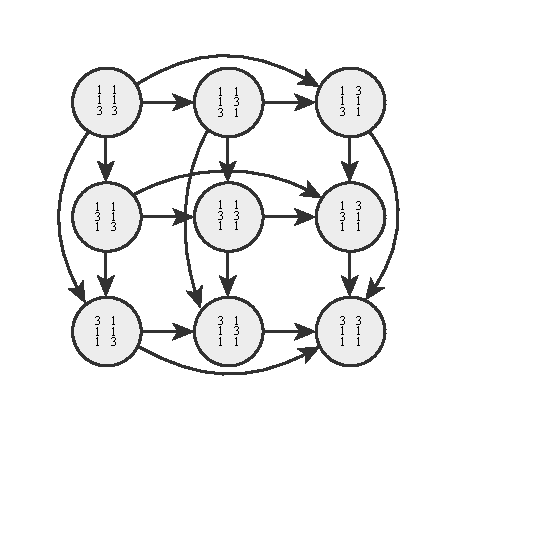
\includegraphics[width=3in]{../figures/diagram6.pdf}
			\caption{A 2-dimensional version of the lattice from Figure \ref{figure-one-dimensional-lattice}.}
			\label{figure-two-dimensional-lattice}
		\end{center}
	\end{figure}

	\begin{proposition}
		\label{proposition-grid-is-lattice}
		Let $(X, \le)$ be a lattice. Let $X^n$ be the set of all $n$-tuples of elements of $X$. Let $\le^n$ be defined as: for all $x, y \in X$ and all $i \in \{1, \ldots, n\}$
		\[
			x \le^n y \iff x_i \le y_i.
		\]
		Then $(X^n, \le^n)$ is a lattice.
	\end{proposition}

	\begin{proof}
		By definition of a lattice, $(X^n, \le^n)$ is a lattice if for any two elements $s, t \in S^n$, $s \join t$ exists and $s \meet t$ exists.

		First we show that $s \join t$ exists. We define $u \in X^n$ such that $u_i = s_i \join t_i$, $\forall i \in \{1, \ldots, n\}$, and we show that $u = s \join t$. Because $u_i = s_i \join t_i$, we have
		\[
			u_i \ge s_i \textrm{ and } u_i \ge s_i
		\]
		so
		\[
			u \ge^n s \textrm{ and } u \ge^n t
		\]
		meaning that $u$ is an upper bound for $s$ and $t$. Suppose there is some $v \in X^n$ which is also an upper bound for $s$ and $t$. Then $\forall i \in \{1, \ldots, n\}$ we have
		\[
			v_i \ge s_i \textrm{ and } v_i \ge t_i
		\]
		so since $u_i = s_i \join t_i$, then $u_i \le v_i$. Therefore $u \le^n v$, i.e. $u$ is the least upper bound of $\{s, t\}$.

		Second we show that $s \meet t$ exists (by the same argument). We define $u \in X^n$ such that $u_i = s_i \meet t_i$, $\forall i \in \{1, \ldots, n\}$, and we show that $u = s \meet t$. Because $u_i = s_i \meet t_i$, we have
		\[
			u_i \le s_i \textrm{ and } u_i \le s_i
		\]
		so
		\[
			u \le^n s \textrm{ and } u \le^n t
		\]
		meaning that $u$ is a lower bound for $s$ and $t$. Suppose there is some $v \in X^n$ which is also a lower bound for $s$ and $t$. Then $\forall i \in \{1, \ldots, n\}$ we have
		\[
			v_i \le s_i \textrm{ and } v_i \le t_i
		\]
		so since $u_i = s_i \meet t_i$, then $u_i \ge v_i$. Therefore $u \ge^n v$, i.e. $u$ is the greatest lower bound of $\{s, t\}$.
	\end{proof}
